\documentclass{acm_proc_article-sp}
\usepackage{algorithmic}
\usepackage{algorithm}
\usepackage{listings}
\usepackage{booktabs}
\usepackage{graphicx}
\begin{document}

\title{Re-Allocation of Resources during Releases \titlenote{Copyright note}}
\numberofauthors{2}
\author{
% 1st. author
\alignauthor
Md Tajmilur Rahman\\
       \affaddr{Concordia University}\\
       \affaddr{Montreal, QC H3G 1M8}\\
       \affaddr{438-932-2288, +1}\\
       \email{mdt\_rahm@encs.concordia.ca}
% 2nd. author
\alignauthor
Peter C. Rigby\\
       \affaddr{Concordia University}\\
       \affaddr{Montreal, QC H3G 1M8}\\
       \affaddr{514-848-2424, +1}\\
       \email{peter.rigby@concordia.ca}
}
\date{20 Oct 2013}
\maketitle
\begin{abstract}
This section will be written at the end.
\end{abstract}
\category{K.6.3}{Software Management}{Software Development, Software Resource Management, Resource Reallocation}
\terms{Experiment, Human Factors, Resource Management, Reallocation}
\keywords{Resource Reallocation, Code Ownership, Defect Density, Software Releases} % NOT required for Proceedings
\section{Introduction}
Software projects are notorious for going over budget and schedule. Rush periods are often get seen before a major release that turn the developers into dinosaurs as Frederick Brooks likens in his benchmark study "The Mythical Man Month" \cite{brooks_mythical}. This "Rush To Release (RTR)" can be prompted either by external forces such as decisions by management to include new features in the release or to release earlier to beat a competitor. Alternatively, the rush may simply be due to inappropriate or unrealistic scheduling. Whatever the reason is it is an obvious. Regardless of the causes, the rush to release stresses developers and often requires developers to work on unusual, high priority or critical areas of the system. In this paper we study how RTR effects project organization and introduces technical debt. We want to propose a method to observe, analyze and summarize the results of revisions found near release. We intend to infer behavior of the developers related to the process around release time. The key research questions that we expect to answer with our methodology are described in section 1.1.

During the merge window, developers are free to provide any change that is ready for release. During the release candinate period, we would expect to see fixs on the files that were changed during the previous merge window. We measure this by comparing the Jac of merge window with the subsequent rc period, compared with the merge window and subsequent merge window.

We observe the developers' working areas to understand the allocation of the resources within an open source software development project to identify that an improper reallocation or inappropriate reorganization causes a disruptive event take place in a software development process. We attempt to identify a project's different release times and calculate the difference between different development periods within a releases to identify which new areas are being worked on and what is the behavior of the developers between normal development period and the period when RTR is prompted before a releases. The historical data from git that we are working on for this purpose will help us to extract a lot of information like calculating the developers' working areas and time-frame of each release as well as different periods in a stable release period. This information will help us to identify the criteria of the resources, their roles and behaviors, code ownership and defect density of the domains they are working in.

We have organized this paper as follows. In Section 2, we describe some background and motivations followed by some summaries of related works in Section 3. Section 4 will describe methodology of our work and the data we are using for this research. In section 5 we will dicuss the results of the findings. Section 6 is going to cover the threats to validity. Finally section 7 will conclude the paper.

\subsection{Research Questions}
We have set our research questions focusing the key properties of software development process, allocation of developers throughout the process, especially for open source software development. First couple of research questions are to understand the basic structure and strategies of the development and release and merging process practiced by Linux. Rest of the questions are to understand the distribution of developers working areas and the behavior of developers in different segments of a release period.

\renewcommand{\labelenumi}{Q\theenumi:}
\begin{enumerate}
\item What is the release process used by the project? \newline
We are going to give a qualitative description of Linux Kernel development in brief to give anser to this question.
\item How many developers are allocated troughout different segments of a release period? \newline
Answer to this question will give us a big picture of Linux Kernel development community as well as the contrubution of developers in different periods within a stable release period.
\item Do developers work on different areas of the system around the time of release? \newline
We want to see if developers are looking at different types of files in the code-base around the time of release which is being considered as the merge period or merge window\cite{linux_kernel}. We are expecting this would be the RTR are in a release time where technical debt may be introduced.
\item How do developers own code around t he system?
Many developers are working on many files. We will find out which files has been churned mostly by which developer so that we can understand how developers are distributed among the system.
\item Are there certain areas of the system that receive increased attention (i.e.\ do developers focus on a smaller set of files around releases)? \newline
To answer this question we will look into the frequency of file churns made into files. Difference or distance of the files between normal development period and the RTR period or merge period of a release.
\end{enumerate}

\section{Background}
There may have lower developers productivity \cite{cataldo_identification, damian_awareness} which may cause inefficient run in the rush moments in a release period. There is a substantial and important body of literature on risk in software engineering. Boehm identified the most important risks encountered by software project managers and described successful risk management practices \cite{boehm_software_risk, keil_framework, boehm_agile}. Some of the risks identified are related to disruptive events, such as the introduction of a new technology, but most are macro risks associated with running a project, such as developing the wrong functionality. General risk mitigation strategies can be difficult to apply to specific disruptive events. There may be various kinds of disruptive events for example, as a release approaches; developers take shortcuts that introduces technical debt. If it is not repaired, the long term quality of the system will suffer. Another example can be placed, if a lead developer who owns an important part of the code-base leaves and if steps to train other developers were not taken, it will become a dead area of the system and will be difficult to modify and maintain. Also often management reorganizes the developers on a company's projects during the rush period around the release time, with the result that developers move to code-bases for which they have less experience. The reorganization introduces new perspectives and expertise that can lead to faster release; however, it can also result in a drop in productivity and the unnecessary re-writing of large portions of the system that the new developers do not understand.
In this paper, we plan to take the measures on this last example among them mentioned above.

\section{Related Works}
Hindle worked on release pattern discovery via partitioning \cite{hindle_release_pattern} to propose an approach to characterize a project's behavior around the time of major and minor releases while we are trying to study the behavior of the development resources around the time of release. In this research they proposed a method of observing, analyzing and summarizing the results of metrics of revisions found near releases. They have characterized a project's behavior around the time of major and minor releases. This is done by partitioning the observed activities like the artiffect check-ins around the dates of major and minor releases, then look for reasonable patterns. Hindle divided the revisions in each release in 4 different classes, Source Code, Testing, Building, and Documentations. On the other hand Cook did an interesting job, he inserted sensors and monitors into the development process but Hindle analyzed the data to understand what happened in the past \cite{cook_automating}. Basically Hindle worked in a reverse way than Cook did. Another research work we would like to mention was done by  Damian where they have worked on the role of domain knowledge and cross functional communication among the OOS development teams \cite{damian_domain}. Posnett did some dual ecological measures of focus in software development \cite{posnett_ecological}. Posnett's measure was for the more general view that unifies developer focus and artifact ownership. He analyzed i) developer artifact contribution to network to a predator-prey food web ii) drew upon ideas from ehology to produce a novel and iii) conceptually unified view of measuring focus and ownership. Another study was done by F. Rahman about the authorship of the code-bases in OSS development \cite{rahman_ownership}.

\section{Methodology and Data}
This section presents our methodology for discovering information which can give us the idea to get the answers to our research questions. We have collected the development history data of Linux kernel. It is a data source containing the the historical data of Linux kernel development since 2005. We are going to present the steps involved in this process and then we will follow up with an application of our methodology in a case study. In order to address our research questions, we obtain key measures of project evolution from the archival data collected from the distributed version contron (DVC) system of Git where all information of the OSS project ``Linux Kernel Development'' is recorded in electronic form. Many other OSS projects archive similar data, so the techniques used here can be replicated on any such project. We used the data elements extracted from the archival source to construct a number of measures on the commit log records to understand the behavior of the developers.

Our methodology can be summarized as: Extracting Data for revisions and releases (Section 4.1); Partitioning the version numbers (Section 4.2); Get time-span between each release (Section 4.3); Calculate developer areas (Section 4.4); Finding code ownership (Section 4.5). Calculating Jaccard Distance for different development areas.

\subsection{Data Extraction}
We went for the VCS of a target project and either mirror the repository or download every revision and commit log history data. From DVCSs such as Git we extract the revisions and release information. We wrote Perl scripts to extract date that was further processed to obtain details. Manual inspection was used to resolve problems and things like that in cases where all automated techniques failed.
We then put them into a database. We have used PSQL database to create tables in, to store our extracted data. These extracted data will be analyzed by us later on. Per each revision the information extracted includes the commit id, tree id, author of the revision, date of revision, the name of the revised file, parent and child info for the revision and the detail log information. Once extraction is completed we are ready to partition the version numbers (Section 4.3) and duration  of each release (Section 4.4).

\subsubsection{Explanation}
A Linux kernel development release version having maximum length of information does look like \textbf{linuxvA.B.C-rcP} where A, B, C, P are numeric. If a release versioning looks like ``linuxv2.6.13'' it tells us that this particular release is the 13th minor release  in the seriese of the 6th major release of kernel version 2. ``linuxv2.6.13\textbf{-rc1}'' says that after the 12th stable minor release had published, development for the next release has been started and rc1 is the first candidate on the way to the next release. It also ensures that next release is going to be another minor release which is ``linuxv2.6.13''. We have last couple of release candidates and the release date for ``linuxv2.6.12'' and first couple of release candidates for ``linuxv3.12'' which is not useful for our calculation. So we are having 340 releases including major, minor, micro and rc; 40 stable releases from ``linuxv2.6.12'' to ``linuxv3.11''. We have total 400441 distinct commits and for 372943 of them have change information for 77082 different files in our hand where we have 14599 developers' working history among 14621 distinct developers. Surprisingly 14569 individual files didn't have any change (addition or deletion) but was being committed at least once. So we found them in our released wise datasets.

\subsection{Finding Release Commits}
As out first step we had to sort out all the commits together those are belonging to any of the releases that we have. We have all 400441 commits in our hand but though we can't plot them into a single time domain to say that these commits are for release 2.6.12 and these are for 2.6.13 and these are for 2.6.14 and so on because commits go on parallelly in git if there are multiple branches. If there are multiple branches, surely there are multiple merges and the commits prior to a crisscross merge are all ancestors of the heads of all subsequent branches \cite{bird_git}. Figure 1 shows how a git DAG looks like having so many crisscross merges in a busy branching snap-shot of the git DAG of Linux Kernel development.
\begin{figure}
\begin{center}
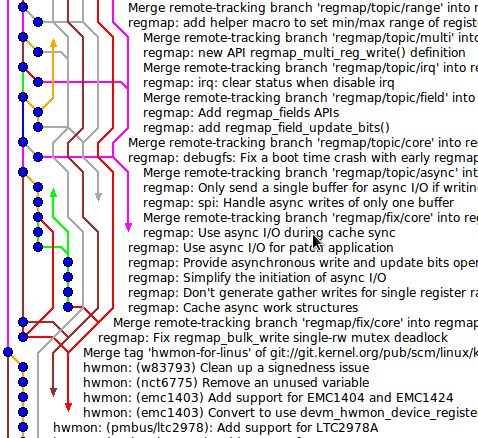
\includegraphics[height=3.5in,width=2.5in]{gitdag.png}
\caption{\small \sl Branching in git DAG for linux kernel development.}
\end{center}
\end{figure}
So it is possible to make a commit months ago from today while several releases may have already been made in the mean time but that commit can belong to any future release. Commits that are being made to a branch may get merged with other branch or the head branch during the release period. This is why we had to track all the way down the trees for each of the 340 releases in the git DAG to find out which commit contributes to which release. We could do this using Git DAG Traversing (GDT) algorithm as shown in Algorithm 1. After applying GDT we collected 381152 out of 400441 commits those are well organized in the git DAG for Linux Kernel development. As we mentioned earlier that we have last couple of release candidates and the release date for ``linuxv2.6.12'' and first couple of release candidates for ``linuxv3.12'' and we are choping out them because we don't have complete data for version 2.6.12-rc as well as 3.12-rc releases, 19289 commits belonging to those releases. So finally we have 381152 commits for 340 releases in our hand to progress our work on.

\begin{algorithm}
\caption{Traverse Git DAG to find Commits within Releases}
\begin{algorithmic}[1]
\REQUIRE
\STATE commit id for all releases
\ENSURE
\FOR{all commits}
\STATE start from new commit, release R
\STATE store commit in ``git\_commit\_release''
\IF{has parent commit}
	\FOR{each parent commit}
		\IF{if parent commit has a release tag}
			\STATE repeat step 1
		\ELSIF{parent commit already stored}
			\STATE compare release versions
			\IF{release version not smaller than R}
				\STATE update existing\_release $\gets$ R
			\ENDIF
		\ELSE
			\STATE store parent commit in ``git\_commit\_release''
			\STATE commit id $\gets$ parent commit id
			\STATE repeat step 3
		\ENDIF
	\ENDFOR
\ELSIF{no parent commit}
	\STATE repeat step 1
\ENDIF
\ENDFOR
\end{algorithmic}
\end{algorithm}

 \subsection{Partitioning Release Numbers}
We stored the extracted git commit log data into the tables git\_commit and git\_revision where all the basic and log information for a particular commit was mentioned in the first table and second one containing which commit belongs to which version of Linux kernel development and change details like path modified, new path created due to the change, how many addition and how many deletion occurred in a particular commit etc. By joining these tables we can easily get the dates of each version and from the version number which is a combination of different types of releases we can get determine which commit belongs to which version and release, and also what type of release that is.

We are getting the release dates with every single commit record. So we can understand which commit belongs to which version of release; is this a major release or minor or micro. Another information we have captured that is \textbf{rc} which means that the particular commit was a release candidate.

\subsection{Time-Span of Releases}
Another information that we require is what are the durations of the releases of Linux kernel development. To achieve that we joined the table in figure 1 and the table ``git\_commit'' which gives us all the dates of commit for each and every release, so we can easily find out the duration between two consecutive releases (all including release candidates RC). This information is more important to us because we need to see what is the general development period and what is the merge which we can treat as RTR period within a release period of time. We also need to understand how developers are working, what is the impact of their changes made in the code-base during a particular release period later on. Table 1 shows a small portion of this information. Preior to calculate the developers' areas in secion 4.4 we require this information.

\begin{table}[ht]
\caption{Different Releases}  % title of Table
\centering 						% used for centering table
\begin{tabular}{c c c c}				% centered columns (4 columns)
\hline\hline						%inserts double horizontal lines
% table heading
Release & Type & Start Date & End Date \\ [0.5ex]
\hline 							% single horizontal line
% inserting body of the table
linuxv2.6.12-rc2 & rc       & - & 2005-04-16 \\
linuxv2.6.12-rc3 & rc       & 2005-04-16 & 2005-04-20 \\
linuxv2.6.12-rc4 & rc       & 2005-04-20 & 2005-05-07 \\
linuxv2.6.12-rc5 & rc       & 2005-05-07 & 2005-05-24 \\
linuxv2.6.12-rc6 & rc       & 2005-05-24 & 2005-06-06 \\
linuxv2.6.12        & micro & 2005-06-06 & 2005-06-17 \\
linuxv2.6.13-rc1 & rc       & 2005-06-17 & 2005-06-29 \\
linuxv2.6.13-rc2 & rc       & 2005-06-29 & 2005-07-05 \\
linuxv2.6.13-rc3 & rc       & 2005-07-05 & 2005-07-13 \\
...			     & ...	   & ... 		     & ...\\
...			     & ...	   & ... 		     & ... \\
...			     & ...	   & ... 		     & ... \\
linuxv3.11            & minor & 2013-08-25 & 2013-09-02 \\
linuxv3.12-rc1     & rc       & 2013-09-02 & 2013-09-16 \\
linuxv3.12-rc2     & rc       & 2013-09-16 & 2013-09-23 \\
linuxv3.12-rc3     & rc       & 2013-09-23 & 2013-09-29 \\
[1ex]							% adds vertical space
\hline 							% inserts single line
\end{tabular}
\label{table:nonlin} 				% is used to refer this table in the text
\end{table}

Note that the very first row has no information for the ``Start Date'' because we don't have any data prior to stable release ``linuxv2.6.12''. From the extraction we found complete records for releases ``linuxv2.6.13'' to ``linuxv2.6.39'' then it is ``linuxv3.0'' to ``linuxv3.11''. Our farther works will be proceeded based on these 40 releases only. As we don't have the complete release information for 3.12 or later and also for 2.6.12 or earlier ones, we are going to not consider them in our farther calculation.

\subsection{Calculate Developers' Area}
Developers are working throughout the release time. Here ``Developers' Area'' (DA) means the files developers work in within a release time. It doesn't refer to the file itself but it is important to understand which files are being touched by which developers. We see that authors are committing files almost everyday throughout a release. We have the commit log data in our hand and we know what is the duration for each and every releases (i.e.\ start and end dates). Now it is possible to find out which commits were made for which files by which developer within a certain time range of a release.

\subsubsection{DA in a Release Period}
We select all the release information from the table where we stored the releases with their corresponding time-span. After that we select author name and other relevant information from the joining of ``git\_revision'' and ``git\_commits'' tables for every release. We insert these information into another table so that we can use the data for our further analysis. A relatively straightforward discipline of Linux Kernel Development team is followed with regard to the merging of patches for each release \cite{linux_kernel}.  At the beginning of each development cycle, the "merge window" is said to be opened.  At that time, code which is deemed to be sufficiently stable (and which is accepted by the development community) is merged into the mainline kernel. The bulk of changes for a new development cycle (and all of the major changes) will be merged during this time, at a rate approaching 1,000 changes ("patches," or "changesets") per day. Strategically linux starts a new kernel release with the merging and fixing to get their development branch ready to start development for the next release. So there are two main segments in a release period, one is merge window or merge period (MP) and another is development window what we are going to call Release Development Period (RDP).

Similarly we have calculated DA in both MP and RDP as described in the following subsections.

\subsubsection{DA in a Merge Period}
Merge Perid can be determined from the previous release (any of major, minor or micro releases) date to the first RC date. For example if the date of release for ``linuxv2.6.12''  is 2005-06-17 and date of pushing the first RC for the next release ``linuxv2.6.13-rc1'' is 2005-06-29 then this time period of of 12 days is being called the merge window \cite{14_kernel} or MP. Table 2 shows some merging periods of different releases.

\begin{table}[ht]
\caption{Release Merging Periods}  % title of Table
\centering 						% used for centering table
\begin{tabular}{c c c c}				% centered columns (4 columns)
\hline\hline						%inserts double horizontal lines
% table heading
Release 			& Start Date		& RC Date \\ [0.5ex]
\hline 							% single horizontal line
% inserting body of the table
linuxv2.6.13		& 2005-06-17	& 2005-06-29 \\
linuxv2.6.14		& 2005-08-28	& 2005-09-12 \\
linuxv2.6.15		& 2005-10-27	& 2005-11-11 \\
linuxv2.6.16		& 2006-01-02	& 2006-01-17 \\
linuxv2.6.17		& 2006-03-20	& 2006-04-02 \\
linuxv2.6.18		& 2006-06-17	& 2006-07-06 \\
linuxv2.6.19		& 2006-09-19	& 2006-10-04 \\
linuxv2.6.20  		& 2006-11-29	& 2006-12-13 \\
linuxv2.6.21		& 2007-02-04	& 2007-02-20 \\
linuxv2.6.22		& 2007-04-25	& 2007-05-12 \\
linuxv2.6.23		& 2007-07-08	& 2007-07-22 \\
linuxv2.6.24		& 2007-10-09	& 2007-10-23 \\
linuxv2.6.25		& 2008-01-24	& 2008-02-10 \\
[1ex]							% adds vertical space
\hline 							% inserts single line
\end{tabular}
\label{table:nonlin} 				% is used to refer this table in the text
\end{table}

We understand DA or Developers' Area is the files in the code-base, developers are working from the dataset that we have in our hand. We have the commit logs and every record says about who committed the file when did he/she worked on the file. If we run an SQL query then we can easily find out for every author and for every particular file how many times it's been committed by an author and what changes (here, addition + deletion = churn) he/she has been made. So we are calculating the DA and storing the information into a table. A part of that table is shown in table 3.

\begin{table}[ht]
\caption{DA in Merge Period}  % title of Table
\centering 						% used for centering table
\begin{tabular}{c c c c}				% centered columns (4 columns)
\hline\hline						%inserts double horizontal lines
% table heading
Author		& File Path			& Commits		& Churn \\ [0.5ex]
\hline 							% single horizontal line
% inserting body of the table
D. S. Miller	& include/.../pci.h		& 1				& 8 \\
V. Hanquez	& arch/.../cpu.c		& 1				& 14 \\
A. Bunk		& drivers/.../shmem.c	& 1				& 2 \\
J. Juhl		& arch/.../generic.c		& 1				& 3 \\
[1ex]							% adds vertical space
\hline 							% inserts single line
\end{tabular}
\label{table:nonlin} 				% is used to refer this table in the text
\end{table}

In this table we see in a merging period inside a release period D. S. Miller has made change in pci.h file only once wich the churn number 8. In the similar way we calculate DA in RDP and RTR period as well.

\subsubsection{DA in a RD Period and RTR}
As like MP we can extract the RDP from the. RDP here in Linux Kernel development process is being considered as from the release date of RC1 (i.e.\ first release candidate opening the gate for the development of the next release) to the next release (major, minor or micro) date. For example if the date of release for ``linuxv2.6.13-rc1'' after releasing ``linuxv2.6.12''  is 2005-06-29 and date of publishing the next release ``linuxv2.6.13'' is 2005-08-28 then this time period of of 60 days is being called the RDP. Table 4 is showing some development periods of different releases.

\begin{table}[ht]
\caption{Release Development Periods}  % title of Table
\centering 						% used for centering table
\begin{tabular}{c c c c}				% centered columns (4 columns)
\hline\hline						%inserts double horizontal lines
% table heading
Release 			& RD Start Date	& Release Date \\ [0.5ex]
\hline 							% single horizontal line
% inserting body of the table
linuxv2.6.13		& 2005-06-29	& 2005-08-28 \\
linuxv2.6.14		& 2005-09-12	& 2005-10-27 \\
linuxv2.6.15		& 2005-11-11	& 2006-01-02 \\
linuxv2.6.16		& 2006-01-17	& 2006-03-20 \\
linuxv2.6.17		& 2006-04-02	& 2006-06-17 \\
linuxv2.6.18		& 2006-07-06	& 2006-09-19 \\
linuxv2.6.19		& 2006-10-04	& 2006-11-29 \\
linuxv2.6.20  		& 2006-12-13	& 2007-02-04 \\
linuxv2.6.21		& 2007-02-20	& 2007-04-25 \\
linuxv2.6.22		& 2007-05-12	& 2007-07-08 \\
linuxv2.6.23		& 2007-07-22	& 2007-10-09 \\
linuxv2.6.24		& 2007-10-23	& 2008-01-24 \\
linuxv2.6.25		& 2008-02-10	& 2008-04-16 \\
[1ex]							% adds vertical space
\hline 							% inserts single line
\end{tabular}
\label{table:nonlin} 				% is used to refer this table in the text
\end{table}

So along these RDs of each release period developers get involved in the development for the next release. As we mentioned earlier RTR may happen as the release approaches. Keeping this in our aim list we noticed an important slot in these RDs of releases. We see in between two consecutive releases there is a merging period of time, after that development starts by pushing RCs and once RC releases stops and it takes some days of time for the preperation to publish the release. We are calling this last part as RTR Period because we asume RTR may happen in this period of time before release. Table 5 represents some releases with their corresponding RTR (i.e.\ from end date to rc and date of release).

\begin{table}[ht]
\caption{RTR Periods}  % title of Table
\centering 						% used for centering table
\begin{tabular}{c c c c}				% centered columns (4 columns)
\hline\hline						%inserts double horizontal lines
% table heading
Release 			& RC End Date	& Release Date	& Days \\ [0.5ex]
\hline 							% single horizontal line
% inserting body of the table
linuxv2.6.13		& 2005-06-29	& 2005-08-28	& 5 \\
linuxv2.6.14		& 2005-09-12	& 2005-10-27	& 8 \\
linuxv2.6.15		& 2005-11-11	& 2006-01-02	& 9 \\
linuxv2.6.16		& 2006-01-17	& 2006-03-20	& 8 \\
linuxv2.6.17		& 2006-04-02	& 2006-06-17	& 12 \\
linuxv2.6.18		& 2006-07-06	& 2006-09-19	& 7 \\
linuxv2.6.19		& 2006-10-04	& 2006-11-29	& 14 \\
linuxv2.6.20  		& 2006-12-13	& 2007-02-04	& 10 \\
linuxv2.6.21		& 2007-02-20	& 2007-04-25	& 7 \\
linuxv2.6.22		& 2007-05-12	& 2007-07-08	& 8 \\
linuxv2.6.23		& 2007-07-22	& 2007-10-09	& 9 \\
linuxv2.6.24		& 2007-10-23	& 2008-01-24	& 5 \\
linuxv2.6.25		& 2008-02-10	& 2008-04-16	& 8 \\
[1ex]							% adds vertical space
\hline 							% inserts single line
\end{tabular}
\label{table:nonlin} 				% is used to refer this table in the text
\end{table}

These information above will help us to answer our first research-question.

\subsection{Finding Code Ownership}
So many developers are working from different development communities. We tried to investigate the "code ownership" \cite{mockus_case_study} evolved in Linux Kernel development. Here code ownership is going to be represented as percentage value. Considering the data that we have for complete releases (``linuxv2.6.12'' to ``linuxv3.11'') we filtered the code files and we found 75138 distinct files that have been worked on. We investigate the total number of commits, total number of churn for each and every file also how many developers contributed for these commits and changes. This information yet does not tell about the ownership. We need to find out ownership for every developers in different development areas in an RP. We already have the collection of developers working in different areas MP, RDP, RTR within an RP and stored them with corresponding file they have worked on, how many commits a developer made to a particular file and how many changes he/she has made. We now update those information with the ownership information. For calculating ownership Equation 1 is applied.
\begin{equation}\omega=\frac{n}{N}*100\end{equation}
Where $\omega$ is the ownership and n is the number of total changes made by an atuthor of a file, N is the total number of changes made for a particular file.
To determine a developer be a owner of a file we considering that if the developer makes changes more than 80\% of the total change that the file has got, then that developer can be treated as a owner of the codes of that file similarly as C. Gutwin did \cite{gutwin_awareness} for finding out the main developers' group for a project. We already mentioned that 14569 individual files didn't have any change (addition or deletion) but was being committed at least once. So we found them in our release wise datasets that's why in addition to Gutwin here considering commits also to determine ownership but only for files without any add or remove lines information. If a file has no addition or deletion information (we are calling it churn) in it's commit log but has beet committed by some one at least once then that or those authors may have the ownership for that file. So the equation 1 becomes like:
\begin{equation} \omega = \left\{ \begin{array}{l l} n/N & \quad \text{if $N > 0$}\\ c/C & \quad \text{if $N = 0$} \end{array} * 100 \right.\end{equation}
Where c is the number of commits made by the author and C is the total number of commits made for the particular file.
We calculate code ownership for all different parts MP, RDP, RTR and also for an entire release period RP. Table 6 represents a part of the data where ownerships is calculated.

\begin{table}[ht]
\caption{Code Ownership in RP}  % title of Table
\centering 						% used for centering table
\begin{tabular}{c c c c}				% centered columns (4 columns)
\hline\hline						%inserts double horizontal lines
% table heading
Author 				& Linuxv		& Path				& $\omega$ (\%) \\ [0.5ex]
\hline 							% single horizontal line
% inserting body of the table
Thomas Gleixner		& 2.6.24		& .../numa\_64.h	& 0.0000\\
Jeff Kirsher			& 3.1		& .../ethtool.c		& 0.0000\\
Sathya Perla			& 2.6.29		& .../hwlib.h		& 100.00\\
Roel Kluin			& 2.6.24		& .../innovator.h 	& 100.00\\
David S. Miller		& 2.6.24		& .../visasm.h 		& 100.00\\
Stephen Hemminger	& 2.6.24		& .../qla3xxx.c	 	& 12.083\\
Randy Dunlap			& 2.6.24		& ...\_core.c 		& 100.00\\
[1ex]							% adds vertical space
\hline 							% inserts single line
\end{tabular}
\label{table:nonlin} 				% is used to refer this table in the text
\end{table}
The example given above is calculated for the developers worked for different files in different releases. Ownership is calculated for all the developers in release periods. In the same way we have calculated what is the ownership value for a developer to a particular file in the merge period (MP) in a release, development period (RDP) in a release and RTR period ind a release.

\section{Preliminary Results}
In this section we present results from several quantitative analysis of the archival data from the Linux Kernel development project. The measures we derive from these data are well-suited to answer our research questions. Once we found different releases and the release periods as well as we calculate the work areas and code ownerships for developers we also want to know what is the difference being created by making changes between two consecutive releases. We want to see what is the difference among the releases also among the different sections MP, RDP, RTR in a release period. To observe this we want to calculate the difference using Jaccard Similarity Coefficient \cite{jaccard_alpine} which is represented by the following equation.
\begin{equation} J(A, B) =\frac{|A \cap B|}{|A \cup B|} \end{equation}
So the Jaccard Distance can be obtained by subtracting the Jaccard coefficient from 1.
\begin{equation} d_j(A, B) = 1 - J(A, B) = \frac{|A \cup B|-|A \cap B|}{|A \cup B|} \end{equation}
Here A and B are two sets. For calculating Jaccard Distance between two releases we are considering the files that have been worked for in a particular release as the set A and files worked for in another release is set B. We found that Jaccard distance between two consecutive releases are not too high. For example jaccard bwteen release ``linuxv2.6.13'' and ``linuxv2.6.14'' is 0.925446 and bwteen ``linuxv2.6.14'' and ``linuxv2.6.15'' is 0.9191968. The higest Jaccard distance we have measured is 0.940 which is between 2.6.20 and 2.6.21 on the other hand the lowest distance is 0.906 between 2.6.30 and 2.6.31. Table 7 shows some Jaccard distances for release pairs and in Table 8 we see the Jaccard distance within the same releases between different perilds MP, RDP and RTR.

\begin{table}[ht]
\caption{Jaccard Distance between Releases}  % title of Table
\centering 						% used for centering table
\begin{tabular}{c c c}				% centered columns (3 columns)
\hline\hline						%inserts double horizontal lines
% table heading
From 				& To		& Jaccard Distance	\\ [0.5ex]
\hline 							% single horizontal line
% inserting body of the table
linuxv2.6.13			& linuxv2.6.14		& 0.925446	\\
linuxv2.6.14			& linuxv2.6.15		& 0.919196	\\
linuxv2.6.15			& linuxv2.6.16		& 0.917945	\\
linuxv2.6.16			& linuxv2.6.17		& 0.916900 	\\
linuxv2.6.17			& linuxv2.6.18		& 0.929941 	\\
linuxv2.6.18			& linuxv2.6.19		& 0.937535	\\
linuxv2.6.19			& linuxv2.6.20		& 0.935265 	\\
linuxv2.6.20			& linuxv2.6.21		& 0.940366 	\\
linuxv2.6.21			& linuxv2.6.22		& 0.920760 	\\
linuxv2.6.22			& linuxv2.6.23		& 0.921652 	\\
linuxv2.6.23			& linuxv2.6.24		& 0.929194 	\\
linuxv2.6.24			& linuxv2.6.25		& 0.910464 	\\
[1ex]							% adds vertical space
\hline 							% inserts single line
\end{tabular}
\label{table:nonlin} 				% is used to refer this table in the text
\end{table}

\begin{table}[ht]
\caption{Jaccard Distance between Releases}  % title of Table
\centering 						% used for centering table
\begin{tabular}{c c c c}				% centered columns (4 columns)
\hline\hline						%inserts double horizontal lines
% table heading
Release 				& J(MP, RDP)		& J(RDP, RTR)	& J(MP, RTR)	\\ [0.5ex]
\hline 							% single horizontal line
% inserting body of the table
linuxv2.6.13			& 0.952060		& 0.921850		& 0.996786 \\
linuxv2.6.14			& 0.958213		& 0.839313		& 0.988072 \\
linuxv2.6.15			& 0.947005		& 0.936153		& 0.996408 \\
linuxv2.6.16			& 0.949774		& 0.919361 		& 0.991275 \\
linuxv2.6.17			& 0.938539		& 0.835925 		& 0.971014 \\
linuxv2.6.18			& 0.946127		& 0.865967		& 0.990750 \\
linuxv2.6.19			& 0.960241		& 0.845649 		& 0.993054 \\
linuxv2.6.20			& 0.967823		& 0.804856 		& 0.995071 \\
linuxv2.6.21			& 0.941798		& 0.835575 		& 0.989031 \\
linuxv2.6.22			& 0.947115		& 0.928818 		& 0.997208 \\
linuxv2.6.23			& 0.939658		& 0.909090 		& 0.995797 \\
linuxv2.6.24			& 0.946806		& 0.871875 		& 0.989284 \\
[1ex]							% adds vertical space
\hline 							% inserts single line
\end{tabular}
\label{table:nonlin} 				% is used to refer this table in the text
\end{table}

In table 8 last three columns representing the Jaccard distance between merge period and release development period, between release development and rush to release period, between merge period and rush to release period respectively.

\section{Conclusions}
This section will be written at the end.
%\end{document}  % This is where a 'short' article might terminate

\section{Acknowledgments}
... ... ...
\bibliographystyle{abbrv}
\bibliography{paper1} 
\appendix
%Appendix A
\section{Headings in Appendices}
Apendix section will be written later with the following subsections may be:
\subsection{Introduction}
...
\subsection{Background and Motivation}
\subsubsection{Related Works}
...
\subsubsection{Methodology and Data}
...
\subsection{Conclusions}
...
\subsection{Acknowledgments}
...

\subsection{References}
... ...

\balancecolumns
\end{document}